\newpage
\chapter{APÉNDICES}
\newpage

\section{PROBLEMAS ENCONTRADOS DURANTE EL DESARROLLO}
El principal problema encontrado fue con las versiones. 
\begin{itemize}
\item El proyecto fue creado con Angular 10, y las versiones compatibles de ciertas librerías con Angular 10 no funcionaban del todo bien, como por ejemplo la galería que quería utilizar inicialmente. Al final encontré librerías adecuadas y compatibles con el proyecto, pero habría sido más sencillo realizar esto si la versión de Angular utilizada fuera la 11 o superior.
\item A la hora de hacer las pruebas unitarias, me encontré con un fallo que salía en cada prueba (``cannot read property 'range' of undefined") cuya solución era actualizar a la última versión de Angular o bajar la versión de NodeJS a una inferior a la 14.5.2. Me decanté por la segunda opción ya que cambiar la versión de Angular con el proyecto casi terminado provocaría muchos problemas.
\end{itemize}
\par Otro problema fue que, al utilizar MySQL, en un principio la base de datos estaba instalada en local en el ordenador con el que trabajaba, por tanto si quería utilizarla desde otro dispositivo tendría que crear de nuevo el servidor MySQL y la base de datos. La solución a esto fue solicitar una máquina Ubuntu a la Escuela, donde instalé el servidor Apache y MySQLServer con la base de datos del sistema.\\
\par Por último, se encontraron varios problemas en el despliegue:
\begin{itemize}
\item Al pasar la aplicación a producción, el archivo \textit{index.html} no localizaba los archivos asociados (\textit{styles.css, resources.js, ...}) por lo que no cargaba la página. Esto fue debido a que, cuando se crea una aplicación y se ejecuta en local, el valor de \textit{base href} es ``/", es decir, una ruta absoluta que apunta a la raíz del sitio. Una vez en producción, esta ruta no coincidía con la de los archivos de la aplicación, por lo que hubo que cambiarlo a una ruta relativa ``./".
\begin{figure}[H]
\centering
\centerline{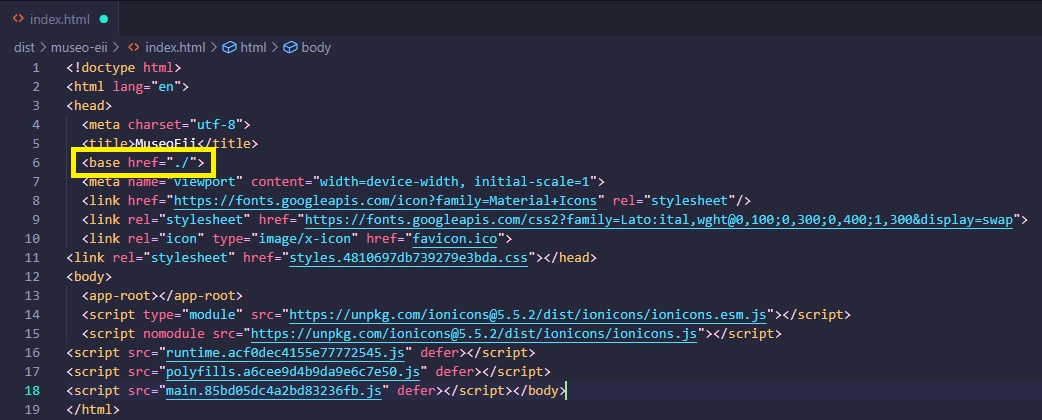
\includegraphics[scale=0.6]{indexhtml}}
\caption{index.html de la aplicación en producción}
\end{figure}
\item Al recargar una página, navegar hacia atrás o indicar una URL directamente en la barra de direcciones, la página no se cargaba y devolvía un error \textit{404: Archivo no encontrado}. Finalmente esto se arregló añadiendo \textit{useHash: true} en el \textit{AppRoutingModule} de la aplicación. Esto cambia la estrategia del enrutador de Angular de \textit{PathLocationStrategy} a \textit{HashLocationStrategy}, y la ruta pasa de \\``http://156.35.163.198/museoeii.com/museum"  \\a ``http://156.35.163.198/museoeii.com/\#/museum". Así el fragmento de la ruta después de la almohadilla no se considera como una página diferente al recargar.
\begin{figure}[H]
\centering
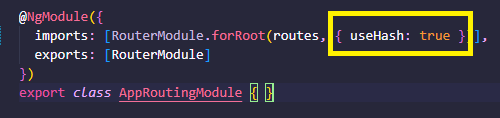
\includegraphics[scale=0.7]{approuting}
\caption{AppRoutingModule de la aplicación}
\end{figure}
\end{itemize}

\newpage
\section{CONCLUSIONES}
Una vez terminado este proyecto, y habiendo desarrollado dos aplicaciones para el museo online y su gestión, se puede decir que ambas cumplen con los objetivos expuestos en el inicio: se pueden añadir y editar piezas y periodos, y toda esta información es presentada al usuario.\par
A nivel personal, estoy contenta con el resultado de este trabajo. Me sentí muy afortunada de poder realizar este TFG, ya que me dio la oportunidad de aprender más sobre desarrollo web con un proyecto cuya idea me gustó desde el momento en el que el tutor habló de su intención de realizar la digitalización del museo. Pude aprender sobre Angular y profundizar un poco más en mis conocimientos de PHP. \par
Me costó más de lo que pude imaginar en un principio, pero es satisfactorio ver el proyecto terminado y funcionando después de tanto trabajo.


\newpage
\section{AMPLIACIONES} 
En esta sección se proponen una serie de ampliaciones del sistema para realizar en un futuro.
\paragraph*{Internacionalización de la base de datos}
Actualmente, la aplicación web permite escoger entre dos idiomas, español e inglés, pero no está completamente internacionalizada. Solo se encuentran traducidos los elementos que se definen directamente en el HTML (títulos, menú de navegación, texto de presentación). Los datos de los periodos y los componentes (descripciones, características, curiosidades, ...) se encuentran solo en español, ya que se leen directamente de la base de datos, en la que se han introducido los datos en este idioma. Por tanto, una posible ampliación sería terminar la internacionalización de la aplicación traduciendo también estos campos leídos de la base de datos.

\paragraph*{Más tipos de componentes}
En la aplicación desarrollada solo se puede añadir y visualizar componentes de tipo genérico o CPUs. Una ampliación a realizar en un futuro será añadir nuevos componentes como, por ejemplo, GPUs. El proyecto actual se ha desarrollado teniendo en cuenta esta posible ampliación, utilizando la interfaz \textit{MyComponent} y dividiendo los componentes de Angular de forma que se puedan añadir nuevas clases realizando los mínimos cambios posibles.

\paragraph*{Generación automática de carteles}
Una ampliación que sería interesante para el proyecto del museo es la generación automática de carteles desde la parte de administración. Esto ayudaría a crear los carteles para el museo físico, ya que pulsando un único botón se aprovecharían los datos ya presentes en la aplicación para generar un cartel informativo del periodo seleccionado y sus respectivas CPUs.

%\newpage
%\section{REFERENCIAS BIBLIOGRÁFICAS}

%\nocite{*} %El comando bibliography enseña solo las referencias que se hayan usado en el texto. Este comando permite "no citar" todas y así que aparezcan.
%\bibliographystyle{ieeetr} 
%\bibliography{references}
